\chapter{Auswertung}
\label{ch:analysis}

In diesem Abschnitt werden die Resultate des Modells analysiert.
Dazu wird der Einfluss jedes Modellparameters einzeln beleuchtet.
Dies soll das Verständnis über die Funktionsweise des Modells erweitern und als Grundlage dienen, das Modell in zukünftigen Arbeiten systematisch zu verbessern.


\section{Einfluss der Anzahl LSTM-Einheiten}
\label{sec:increase-lstm}

Die Erhöhung der Anzahl Zellen scheint einen positiven Effekt auf den Anteil lesbarer Wörter zu haben (Tabelle \ref{tab:results-of-various-configurations-layers-units}).
Die durchschnittliche Wortlänge nimmt allerdings geringfügig ab.
Diese Auswirkungen könnten darauf zurückzuführen sein, dass durch die zusätzliche Anzahl an Zellen mehr Informationen bzw. mehr valide Buchstabenkombinationen gespeichert werden können.
Umgekehrt könnte der höhere Anteil unlesbarer bzw. nicht-verwendbarer Wörter bei weniger Zellen damit erklärt werden,
dass das Modell – aufgrund des begrenzten Speicherplatzes – bei einigen Wörtern und Buchstabenfolgen Kompromisse eingehen muss.
Allerdings hat die höhere Lesbarkeit bei mehr Zellen den Effekt, dass die Originalität sinkt.
Dadurch dass ein grösserer Anteil Wörter korrekt geschrieben wird, steigt auch die Wahrscheinlichkeit, dass das Modell Sequenzen generiert, die genau so im Trainingssatz vorkommen.

Im Weiteren ist zu beobachten, dass die Anzahl insgesamt erzeugter Wörter leicht abnimmt, wenn die Zellenzahl erhöht wird (z.B. von 6'885 auf 6'383 von 64 auf 512 Zellen).
Diese Beobachtung kann auch nach mehreren Durchläufen gemacht werden, sowohl bei einfachen wie auch bei mehrschichtigen Netzen.
Die Anzahl der Zellen scheint also eine Auswirkung auf die «Redefreudigkeit» des Modells zu haben.
Deutlich ist dieser Effekt indes bei den dreischichtigen Konfigurationen zu erkennen (von 10'094 auf 6'848 Wörter).
Möglicherweise spielt auch hier der Kompromisszwang eine Rolle.
Hat das Modell weniger Speicherplatz zur Verfügung, so muss es öfters einen Kompromiss zwischen der Stoppmarke und einem beliebigen anderen Zeichen eingehen.
Im ausgegebenen Wahrscheinlichkeitsvektor für das prognostizierte nächste Zeichen äussert sich das so, dass der Unterschied in der Wahrscheinlichkeit zwischen einer Stoppmarke sowie einem
anderen Zeichen geringer ist als in einem Netz mit mehr Speicherplatz bzw. Zellen.
Der Effekt äussert sich sodann auch in der durchschnittlichen Namenslänge.

\section{Einfluss der Netztiefe}
\label{sec:increase-lstm-layers}

Ein gutes Modell sollte fähig sein, von den Trainingsdaten zu abstrahieren.
Dies kann u.a. mit mehrschichtigen («deep») Netzen erreicht werden.
Ein typischer Anwendungsfall liegt z.B. bei sog. «Convoluted Neural Networks» (dt. «überlagerte Neuronale Netzwerke») vor.
Hierbei werden mehrere Netzschichten verwendet, um von einzelnen Informationen (z.B. Pixel) über mehrere
Schichten (Kante, Rechteck, Tür, Haus, …) zu abstrahieren, ähnlich der menschlichen Wahrnehmung\footnote{vgl. https://towardsdatascience.com/a-comprehensive-guide-to-convolutional-neural-networks-the-eli5-way-3bd2b1164a53}.
Ein Abstraktionskonzept für das Sprachmodell zu entwerfen würde den Rahmen dieser Arbeit sprengen.
Trotzdem soll der Effekt der Mehrschichtigkeit untersucht werden.

Wie Tabelle \ref{tab:results-of-various-configurations-layers-units} zeigt, scheint sich die Mehrschichtigkeit
vor allem in der Anzahl erzeugter Wörter nieder zu schlagen.
Am deutlichsten ist das bei den 64-Zellen-Netzen zu beobachten (6'885 Wörter zu 10'094 Wörter).
Womöglich lernt das Modell durch die zusätzlichen Schichten längere Sequenzen.
Die durchschnittliche Namenslänge scheint mit der erhöhten Anzahl erzeugter Wörter zu korrelieren.
Interessant für die Qualität der erzeugten Sequenzen dürfte der zeitgleiche leichte Anstieg im Anteil lesbarer Wörter sowie der Originalität sein.
Das Modell ist mit mehreren Schichten anscheinend fähig, Wörter häufiger korrekt wiederzugeben und zudem einzigartigere Sequenzen zu erzeugen.

Je umfangreicher und komplexer ein Modell aufgebaut ist, desto höher ist allerdings die Gefahr, dass sich das Modell zu stark an die Trainingsdaten anpasst («Overfitting»).
Ist dies der Fall, so sinkt die Fähigkeit des Modells, von den Trainingsdaten zu abstrahieren und hat eine höhere Wahrscheinlichkeit, ebendiese zu erzeugen.
Eine einfache und überraschend effektive Möglichkeit, ein tiefes Netz zu «regulieren» und von den Trainingsdaten zu lösen, bietet die «Dropout»-Methode.
Dabei wird bei jedem Trainingsschritt zufällig ein Anteil («Dropout-Rate») der Zellen ausgeschaltet.
Das Netz muss quasi lernen, mit Ausfällen umzugehen.
Es wird dadurch robuster\autocite{JMLR:v15:srivastava14a}.
Die Auswirkungen der Dropout-Raten 15\% sowie 60\% sind Tabelle \ref{tab:results-of-various-configurations-dropout} zu entnehmen.
Der Effekt scheint beim 512-Zellen-Netz sehr gering zu sein.
Der Anteil lesbarer Wörter steigt leicht an, bei fast gleichbleibender Originalität.
Allerdings steigt die Wiederholungsrate leicht an.
Möglicherweise ist dieser Effekt damit erklärbar, dass das Modell zwar effektiv etwas robuster wird und einen höheren Anteil lesbarer Wörter erzeugt.
Allerdings wird das Modell auch zurückhaltender und wiederholt etwas mehr Erzeugnisse, weil Zellen beim erhöhten Ausfall von Nachbarzellen einspringen müssen und somit einen Teil der Aufgabe der ausgefallenen Zellen übernehmen.
Gravierend ist eine erhöhte Dropout-Rate allerdings für das 64-Zellen-Modell.
Hier dürfte nun der Ausfall dermassen hoch sein, dass das Modell in seiner Lernfähigkeit zu sehr eingeschränkt wird und kein nachhaltiges Sprachmodell aufbauen kann.
Diese Beobachtungen waren in mehreren Versuchen reproduzierbar.


\section{Unterschiedlicher Umfang der Trainingsdaten}
\label{sec:increase-num-dataset}

Wird das Modell nur mit einem Viertel des Datensatzes trainiert, so scheint der Wortschatz begrenzt zu sein.
Wird das Modell zweimal mit dem gesamten Datensatz trainiert, so ist der Wortschatz umfangreich.
Dies äussert sich deutlich im Anteil lesbarer Wörter.
So ist in beiden Modellkonfigurationen ein deutlicher Anstieg (z.B. von 59.92\% auf 85.03\% bei 512 Units und 3 Schichten) zu sehen.
Hat das Modell also ein längeres Training bzw. einen grösseren und vielfältigeren Umfang des Trainingsdatensatzes zur Verfügung, so
schreibt es häufiger Wörter korrekt.
Interessant ist allerdings, dass die Originalität sowie Repetition mit zunehmender Trainingsgrösse abnimmt.
Dies kann damit erklärt werden, dass das Modell bei zu häufigem Training mit denselben Daten in den Bereich des Overfittings gerät.
Der Effekt ist besonders beim 512-Units Netz zu sehen, wo die Repetitionsrate auf 5\% steigt und die Originalität auf 84.89\% sinkt.
Das Modell gibt also bedeutend häufiger Namen aus dem Trainingsset wieder.


\section{Einbezug des Steuerparameters}
\label{sec:including-years}

Der Einsatz unterschiedlicher Jahreszahlen (Tabelle \ref{tab:results-of-various-years}) als Steuerparameter scheint keinen Unterschied auszumachen.
Allenfalls könnte spekuliert werden, dass der Anteil fremdsprachiger Wörter (Französisch, Italienisch, Deutsch, …) um 2000 höher ausfallen müsste,
weil der Einfluss internationaler Küche durch die Globalisierung stärker ist.
Allerdings ist der Unterschied in den erzeugten Sequenzen verschwindend gering.
Wird der Datensatz nach Jahr des ersten Erscheinens sortiert, so könnte der Eindruck entstehen,
dass exotisch klingende Namen tendentiell auch zeitnahe wieder verschwinden, während zeitlos klingende
Namen eher eine höhere «Lebensdauer» aufweisen (siehe Tabelle \ref{tab:data-1900}).
Wird die Verteilung der Zeitspannen analysiert (siehe Abb.\ref{fig:hist-dates-datespans}) so ist jedoch klar ersichtlich,
dass annähernd alle Einträge eine Zeitspanne von 0 bis 2 Jahre aufweisen.
Deshalb ist es unwahrscheinlich, dass die Zeitspanne zusammen mit einem frühen Eintrittsjahr als Mass für einen
aussergewöhnlichen Namen herangezogen werden kann.
Wäre dies der Fall, so müsste der Grossteil der generierten Namen ebenfalls exotisch klingen, da die meisten Datensätze
um das Jahr 1920 angesiedelt sind (gemäss Histogramm in Abb. \ref{fig:hist-dates-dates})
Somit kann die mangelnde Unterschiedlichkeit bei den Jahreszahlen nur darauf zurückgeführt werden, dass bereits
der Datensatz keine klaren Unterschiede in der Sprache aufweist.
Anders als beispielsweise bei \autocite{robertson}, bei dem die Personennamen klaren Mustern folgen und somit deutlicher
den einzelnen Sprachen zugeschrieben werden können (Russische Namen enden z.B. häufig auf «..ov»).
Zudem ist der Sprachstil wohl eher in längeren Sätzen kennzeichnend für eine bestimmte Epoche, weniger aber in kurzen und
grammatikalisch niederkomplexen Begriffen wie das eben bei den Gerichten der Fall ist.
Beste Beispiele für deutliche Sprachstile sind der Shakespeare-Generator\footnote{http://karpathy.github.io/2015/05/21/rnn-effectiveness/} sowie DeepDrumpf\footnote{https://twitter.com/deepdrumpf}.

Ein Unterschied könnte allenfalls in den Zutaten der Speisen ausgemacht werden.
Beispielsweise wäre eine Hypothese, dass der Anteil einfacher und günstiger Zutaten wie Kartoffeln um 1900 höher ist, weil
die Kaufkraft und die gastronomische Affinität der Gesellschaft damals niedriger waren.
Dies zu untersuchen erfordert allerdings sehr viel manuellen Aufwand, was ausserhalb des zeitlichen Rahmens dieser Arbeit liegt.

Stattdessen wurde per \gls{feature-engineering} ein Steuerparameter erstellt, der vegetarische von nicht-vegetarischen Gerichten unterscheidet.
Die Klassifizierung wurde durch eine einfache (und unvollständige), manuell erstellte Liste von Fleisch bezeichnenden Wörtern wie z.B. «Chicken» erreicht.
Die Tabelle \ref{tab:results-of-various-vegetarian} zeigt, dass der Einfluss des Steuerparameters nun durchaus gegeben ist, insbesondere wenn beachtet wird,
dass der Anteil nicht-vegetarischer Gerichte im Datensatz gerade mal 7.5\% beträgt.

Interessant zu beobachten ist die Abnahme der «vegetarischen Verstösse» wenn das Modell mehr Schichten zur Verfügung hat.
Dies könnte wiederum damit zusammenhängen, dass die Abstraktionsfähigkeit des Modells durch Schichten zunimmt.

\begin{figure}
    \centering
    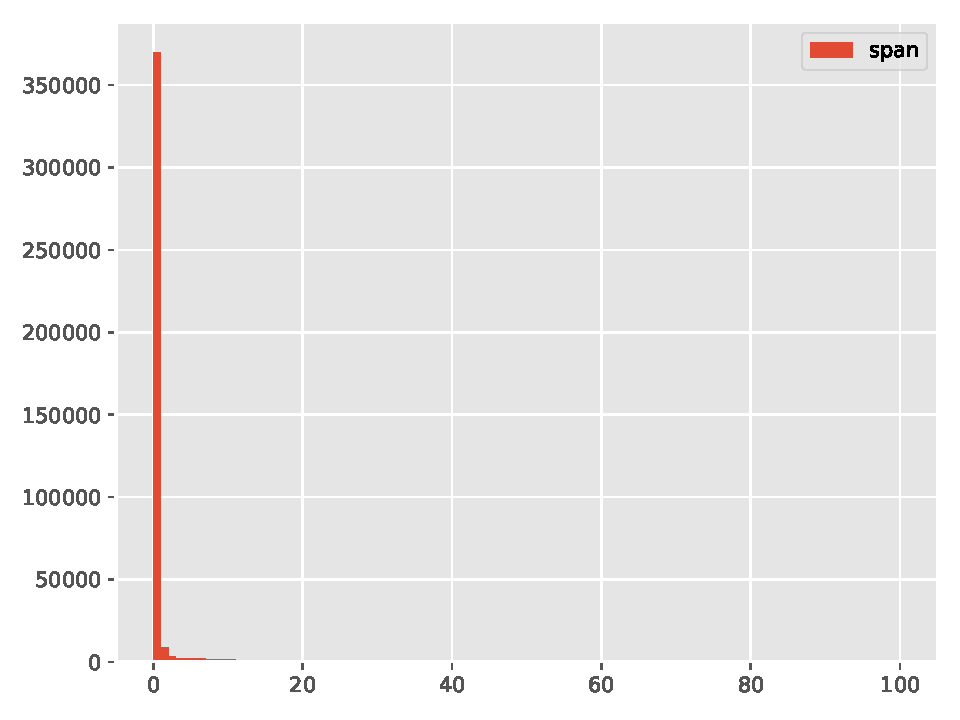
\includegraphics[width=0.75\linewidth]{images/analysis/histogram-datespans.pdf}
    \caption{Verteilung zeitlicher Spannweiten}
    \label{fig:hist-dates-datespans}
\end{figure}



\begin{center}
    \begin{table}
        \centering
        \small
        \begin{tabular}{ |l|l|l|l| }

            \hline
            \textbf{id} & \textbf{name} & \textbf{first\_appeared} & \textbf{last\_appeared} \\
            \hline
            2506 & Egg Sandwich & 1900 & 1965 \\
            2545 & Home-made apple pie & 1900 & 1962 \\
            39540 & Sommerische Gansebrust w. Salad & 1900 & 1900 \\
            510277 & Calf Brains, Liver and Bacon & 1900 & 1900 \\
            510944 & Planked Shad, à la maître d'hotel & 1900 & 1900 \\
            \hline
        \end{tabular} \\

        \caption{Zeitgebundene und zeitlose Gerichte}
        \label{tab:data-1900}
    \end{table}
\end{center}

\section{Praxistauglichkeit \& subjektive Bewertung der Ausgabe}
\label{sub:in-practice}

Das beschriebene und implementiert Neuronale Netz ist relativ einfach und erzeugt trotzdem beachtenswerte Resultate.
Dennoch reicht es nicht aus, die erzeugten Sequenzen nur anhand von Statistiken zu bewerten.
Zumindest ein hoher Lesbarkeits-Wert dürfte als gute Vorbedingung für die Verwendbarkeit gelten.
Subjektiv betrachtet sollen hier einige der erzeugten Begriffe beispielhaft interpretiert werden.
Eine \textbf{«American Special Cream»} könnte als BBQ-Erweiterung einer üblichen Kartoffelsuppe neu umgesetzt werden.
Ein \textbf{«Boiled sea bass a la truffle»}, also gekochter Barsch mit Trüffel
Vielleicht als Suppe?
\textbf{Chicken, Vanilla Puree with Cream, Honey Mayonnaise}: Ein Gericht der Gegensätze, von salzig bis süss.
Allerdings ist Chicken Sweet\&Sour ein weltweit beliebtes Gericht, möglicherweise könnte ein Vanille-Einschlag neue Frische bringen.
\textbf{Deviled Pineapple Cheese}: Ein feuriger Käse mit süss-exotischer Note. \textbf{Fruits or Cereal Salad}: Könnte auch mit Müsli verwechselt werden.
Jedoch sind vollwertige Salate im Trend und werden gerne als leichtes Mittagsessen bestellt.
Warum nicht die Vielfältigkeit in Getreidesorten in einem Salatgericht feiern?
\textbf{Home Made Potatoes}: Wie sehen hausgemachte Kartoffel aus? Haben sie eine ungewöhnliche Form? Sind sie quadratisch statt rund? Sind sie mit Plätzchen-Förmchen ausgestochen? \textbf{Queen Mary Ice Cream}: Ein Eis in Form eines Kreuztfahrtschiffs
\textbf{Cold Fried Filet of Flounder, Buttered Carrots and Cole Slaw}: Wie wird eine Flunder kalt gebraten? Mit Stickstoff? Molekularküche?

Selbstverständlich eignen sich längst nicht alle erzeugten Sequenzen als echtes Gericht, aber sie regen die Kreativität auf jeden Fall an.
Nicht zuletzt muss auch nicht jeder Vorschlag zwingend als Gericht aufgefasst werden.
Erzeugnisse wie \textbf{«All White Fruits»}, \textbf{«Orange or Pink»} deuten eher auf ein ganzes Dinner-Thema hin, während \textbf{Steak de veau a la mode, crackers} durch seine freche Umzinglung der französischen Sprache revolutionäre Töne anschlägt.
